\chapter{Practical implementation of the network interface}
%=================================================================================================
\section{Project goals}

Following project goals were defined while constructing the practical solution: 

\begin{itemize}
    \item [1)] The implementation will consist of a wired network interface using Ethernet and wireless network interface using ESP8266 module;
    \item [2)] The IoT module will receive the network information such as its assigned IP address, subnetwork mask and gateway IP via DHCP service;
    \item [3)] Solution will allow to establish communication with the device using the \emph{ping} command;
    \item [4)] Solution will offer an echo server which will relay back messages received by the IoT module via TCP protocol back to the sender.
\end{itemize}

%=================================================================================================
\section{Chosen components}
\subsection{Hardware platform}

Due to the already available physical implementation for 8P8C socket and wide availability of reference materials such as documentation and resources produced by the community, Nucleo-F429ZI by ST Microelectronics was chosen as the target hardware platform. In order to implement the wireless interface, the aforementioned ESP8266 module was used due to its small cost.

\subsection{Environment and programming language}

During the analysis of available resources a decision was undertaken to pick STM32\dywiz CubeIDE which is the dedicated environment for the chosen hardware platform, as the IDE of choice. This is a result of the availability of embedded configuration tools, which allow for configuring selected parameters of the hardware platform without the need to manually manipulate the registers of the microcontroller. The programming language was determined to be C.

\subsection{Verification methods of the system functionality}

Verification of the system functionality will happen in a two-step process. First step includes transferring information about the IoT module, such as its IP address, subnetwork mask and gateway address via a virtual serial port. Second step consists of an attempt to communicate with the module via \emph{ping} command and communication with the implemented echo server using Hercules SETUP Utility software, which allows communication using the TCP protocol. 

%=================================================================================================
\section{Hardware implementation}

\subsection{Ethernet interface}

Thanks to the selected hardware platform, the hardware implementation was already done in-factory on the Nucleo-F429ZI board. The board contains soldered in 8P8C connector with designated RMII interface, as presented on figure 4.1.

\begin{figure}[!ht]
    \centering
    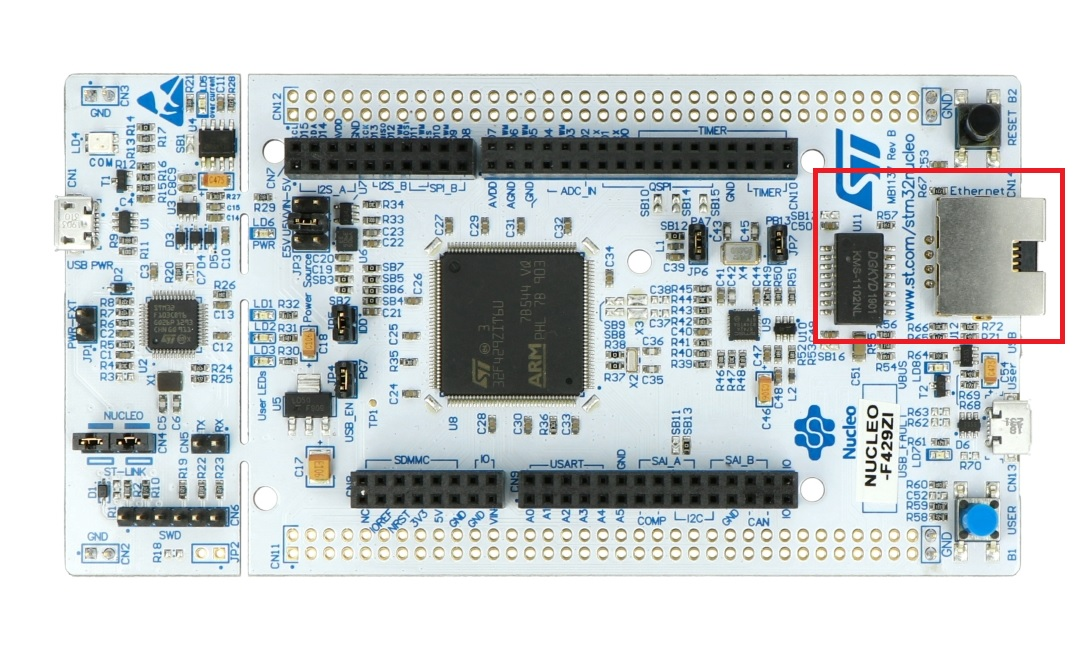
\includegraphics[width=120mm]{Rysunki/Rozdzial4/nucleo 8p8c.jpg}
    \caption{8P8C connector present on the Nucleo-F429ZI board}
    \label{fig:my_label}
\end{figure}

\subsection{Wireless interface}

In order to communicate with the ESP8266 module, an USART6 serial interface of the STM32-F429ZI microcontroller was used. It is present at pins PC6 and PC7. Additionally a PB3 pin was used in order to provide logical high level to the \emph{enable} input pin of the ESP8266. Figure 4.2 shows the schematic of the connections.

\begin{figure}[!ht]
    \centering
    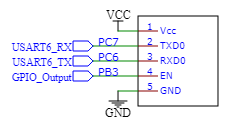
\includegraphics{Rysunki/Rozdzial4/schemat_esp8266.png}
    \caption{ESP8266 connection schematic}
    \label{fig:my_label}
\end{figure}

%=================================================================================================
\section{Software implementation}

\subsection{Ethernet interface}

The first step of the implementation consisted of initializing the Ethernet interface allowing for correct transmission of the \emph{ping} packet and to signalize the state of the connection via an LED.

Initialization process started by launching the STM32CubeIDE environment and creating a new project selecting STM32L429ZI microcontroller. Figure 4.3 shows the microcontroller platform selection, and figure 4.4 options of the created project.

\begin{figure}[!ht]
    \centering
    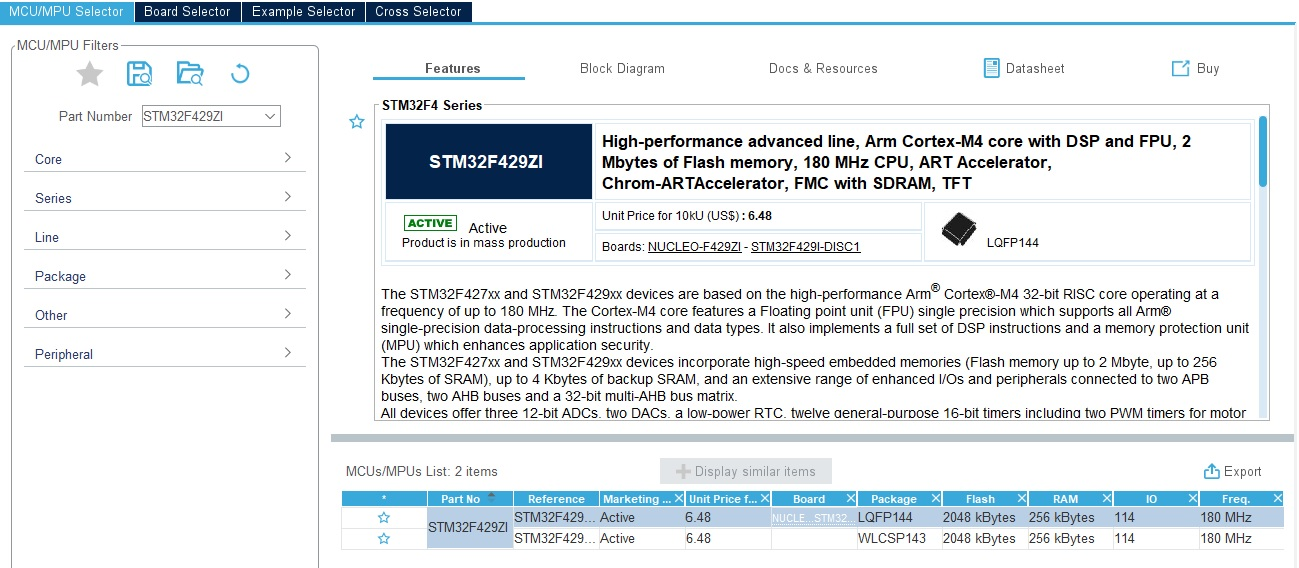
\includegraphics[width=155mm]{Rysunki/Rozdzial4/wybór mikrokontrolera.jpg}
    \caption{Microcontroller selection in STM32CubeIDE}
    \label{fig:my_label}
\end{figure}

\begin{figure}[!ht]
    \centering
    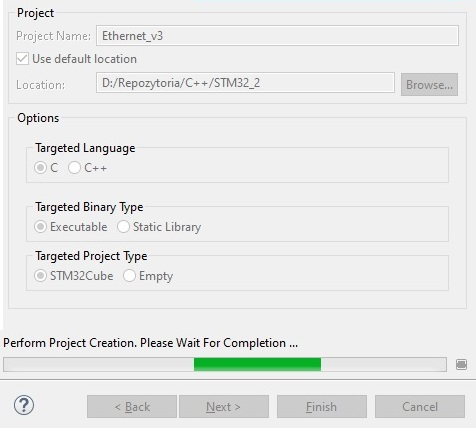
\includegraphics[width=80mm]{Rysunki/Rozdzial4/utworzenie projektu.jpg}
    \caption{Creating the project}
    \label{fig:my_label}
\end{figure}

\newpage
The clock signal provided by ST-LINK module being an embedded part of the Nucleo-F429ZI board was used as the system clock. In order to achieve this, High Speed Clock in the RRC tab needed to be set to BYPASS, which was showcased by the figure 4.5. Resulting configuration of the clocking signal was presented on figure 4.6.

\begin{figure}[!ht]
    \centering
    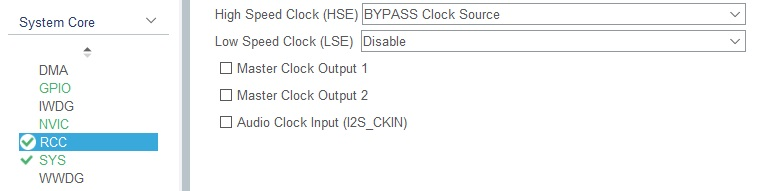
\includegraphics[width=120mm]{Rysunki/Rozdzial4/tryb bypass.jpg}
    \caption{Switching the HSE clock into BYPASS mode}
    \label{fig:my_label}
\end{figure}

\begin{figure}[!ht]
    \centering
    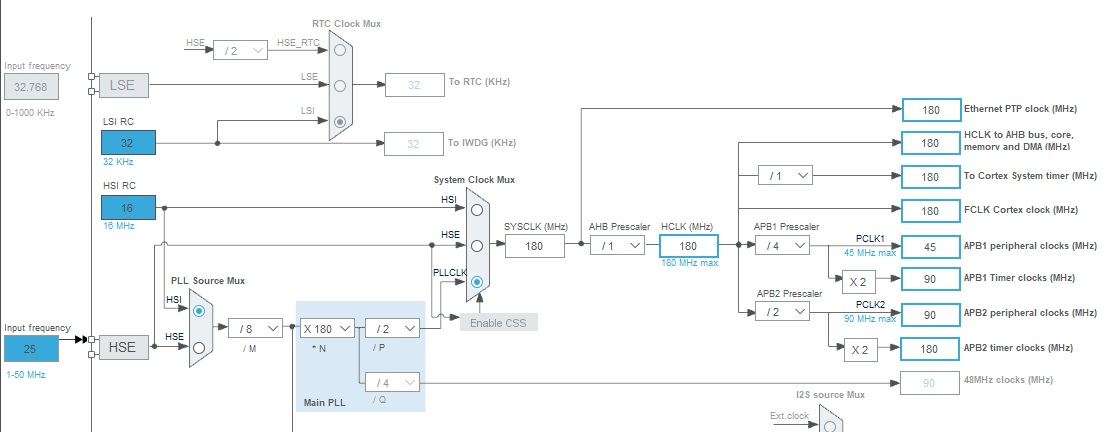
\includegraphics[width=155mm]{Rysunki/Rozdzial4/clock_signal_bypass.jpg}
    \caption{Configuring clocking signal after switching HSE to BYPASS mode}
    \label{fig:my_label}
\end{figure}

\newpage
The Ethernet interface needs to be initially configured in the \emph{Connectivity} tab, setting its mode to RMII. It is a result of the Nucleo-429ZI board structure, in which the Ethernet connection is realized using RMII interface. The default MAC address of the device is equal to 00:80:E1:00:00:00. During the setup of default values via a configurator, the PHY address of the device was assigned as 1. It needed to be changed to 0. The results were shown on figures 4.7 and 4.8.


\begin{figure}[!ht]
    \centering
    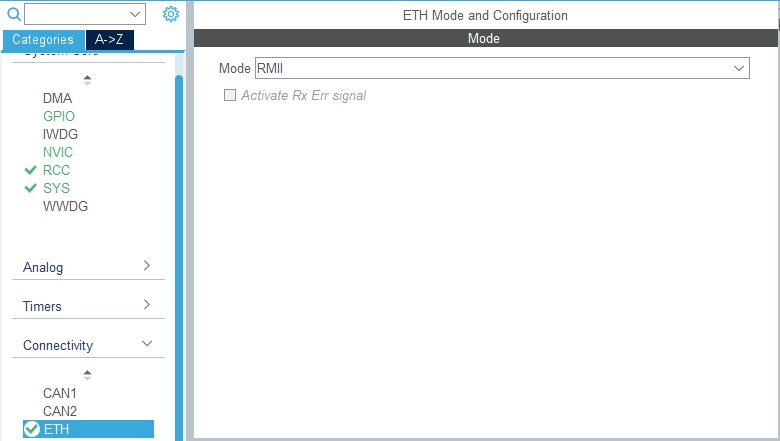
\includegraphics[width=120mm]{Rysunki/Rozdzial4/rmii1.jpg}
    \caption{Assigning RMII mode to the Ethernet interface}
    \label{fig:my_label}
\end{figure}

\begin{figure}[!ht]
    \centering
    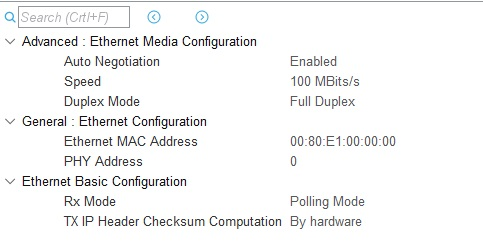
\includegraphics[width=120mm]{Rysunki/Rozdzial4/rmii2.jpg}
    \caption{Target values of RMII parameters}
    \label{fig:my_label}
\end{figure}

Due to the connections present on the Nucleo-F429ZI board in accordance to the table presented in the manufacturer documentation \cite{nucleo-manual} the output pins of the microcontroller were assigned in a way showcased in table 4.1. The RMII interface connection schematics are presented by figure 4.9.

\newpage

\begin{figure}[!ht]
    \centering
    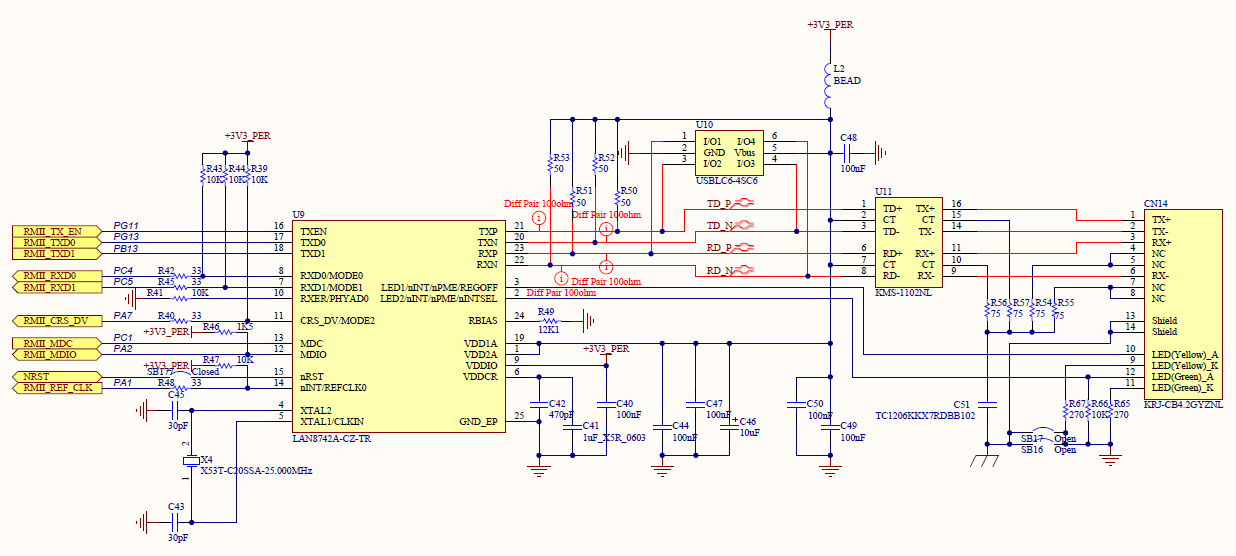
\includegraphics[width=140mm]{Rysunki/Rozdzial4/schemat_RMII.png}
    \caption{RMII interface connection schematics}
    \label{fig:my_label}
\end{figure}

{\centering

\begin{longtable}{c|c}
    \caption{Output line assignment} \\
    Pin name & Functionality \\
    \hline
    PA1 & ETH\texttt{\char`_}REF\texttt{\char`_}CLK \\
    PA2 & ETH\texttt{\char`_}MDIO \\
    PA7 & ETH\texttt{\char`_}CRS\texttt{\char`_}DV \\
    PC4 & ETH\texttt{\char`_}RXD0 \\
    PC5 & ETH\texttt{\char`_}RXD1 \\
    PG11 & ETH\texttt{\char`_}TX\texttt{\char`_}EN \\
    PG13 & ETH\texttt{\char`_}TXD0 \\
    PB13 & ETH\texttt{\char`_}TXD1 \\
    PB14 & Red LED \\
    PB0 & Green LED \\
    PB7 & Blue LED \\
    Pin name & Functionality \\
    \hline
    PD9 & RX line of virtual serial port USART3 \\
    PD8 & TX line of virtual serial port USART3
    \label{tab:my_label}
\end{longtable}
}

The next step included configuring the LwIP stacked used for operating the TCP/IP stack protocols. In order to do that, user needs to proceed to the \emph{Middleware} tab as shown on figure 4.10, where the user gains access to various software for selected microcontroller, such as the LwIP stack or freeRTOS real time operating system. The LwIP stack is characterized by big selection of configuration options. In the implementation for the needs of this dissertation, majority of the configuration can be left as default. User needs to make sure however that the LWIP\texttt{\char`_}NETIF\texttt{\char`_}LINK\texttt{\char`_}CALL-BACK, which designates a function called when the Ethernet connector is plugged in to 8P8C socket, is enabled, as shown on figure 4.11. 

\begin{figure}[!ht]
    \centering
    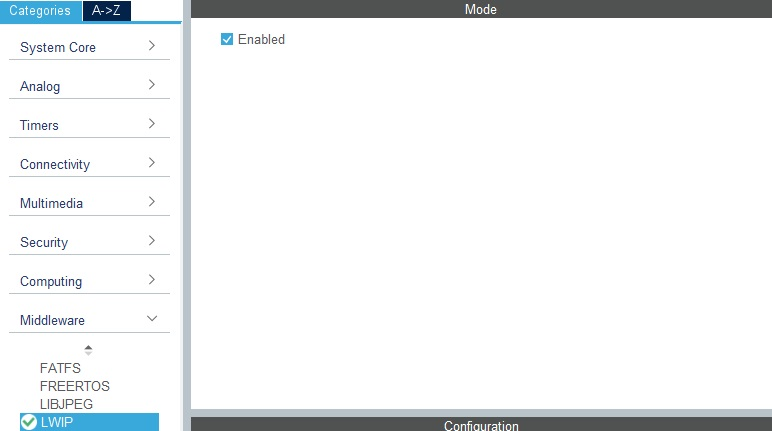
\includegraphics[width=120mm]{Rysunki/Rozdzial4/middleware_lwip.jpg}
    \caption{Enabling LwIP stack}
    \label{fig:my_label}
\end{figure}

\begin{figure}[!ht]
    \centering
    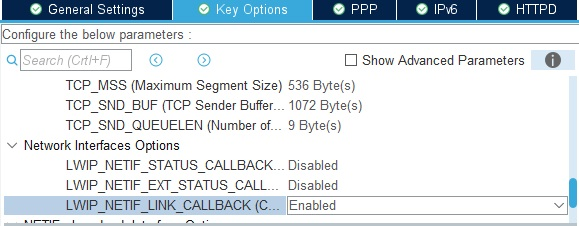
\includegraphics[width=100mm]{Rysunki/Rozdzial4/middleware_lwip_2.jpg}
    \caption{LWIP\texttt{\char`_}NETIF\texttt{\char`_}LINK\texttt{\char`_}CALLBACK option}
    \label{fig:my_label}
\end{figure}

\newpage
Using the \emph{Clock Configuration} tab, the Ethernet clock signal was set to the frequency of 180 MHz, via the PLL loop and correct prescalers, as presented by figure 4.12.

\begin{figure}[!ht]
    \centering
    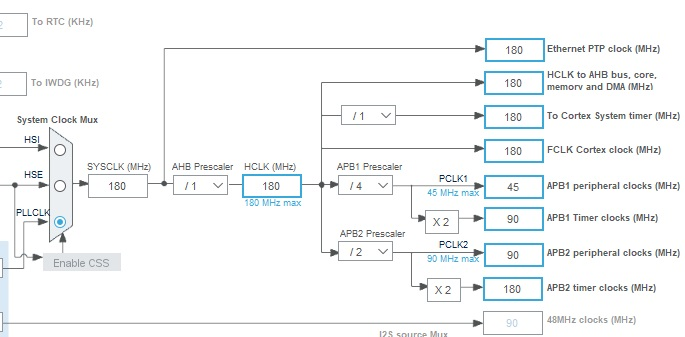
\includegraphics[width=120mm]{Rysunki/Rozdzial4/clock_config.jpg}
    \caption{Clock configuration}
    \label{fig:my_label}
\end{figure}

The follow up included generating the code and its modification. During the implementation of the echo server using the LwIP stack and modification of the \textit{MX\char`_LWIP\char`_Process()} function, it was decided to use a sample implementation by a korean Naver blog user nicknamed eziya76 \cite{eziya76}.

\cppcode{Listingi/Ethernet_main.c}{Ethernet implementation \textit{main()} function}

Listing 4.1 presents the contents of the \textit{main()} function for the project implementing the Ethernet interface. Part of this function was generated via the code generator based on the STM32CubeIDE environment configuration.

In order to store and format information regarding the connection, such as the IP address, subnetwork mask, gateway address, MAC address and connection status, 5 globally available buffers were created. This information is transmitted to the overseeing computer via USART3 serial port inside the \textit{notify\char`_dhcp\char`_status()} function.

The \textit{MX\char`_LWIP\char`_Process()} function takes care of receiving the dynamic IP address from the DHCP server enabled in the router and was presented on listing 4.2. The echo server is initialized in the \textit{init\char`_echo()}, repeating a copy of received message to the sender. Listing 4.3 showcases implementation of the \textit{notify\char`_dhcp\char`_status()} function. Listings 4.4 - 4.7 picture the implementation of functions that process information about connection and MAC address into a character string.

\cppcode{Listingi/LWIP_Process.c}{MX\textit{\char`_}LWIP\textit{\char`_}Process() function}

\newpage
\cppcode{Listingi/notify_dhcp_status.c}{Connection state overseeing function}

\cppcode{Listingi/parse_ip.c}{Function processing the IP address}

\cppcode{Listingi/parse_mask.c}{Function processing the subnetwork mask}

\cppcode{Listingi/parse_gateway.c}{Function processing the gateway address}

\newpage
\cppcode{Listingi/send_mac_address.c}{Function transferring the MAC address during the start of the device}

In order to control the echo server, a \textit{echo\char`_info} structure was created, which stores information regarding the connection status, retransmission count, pointer to the pcb structure of the LwIP stack and a pointer to the transceiveing buffer. Additionally, an enumerating type was created which allows to use connection state names instead of numerical values. Aforementioned elements were placed in a header file listed on listing 4.8. 

\cppcode{Listingi/echo.h}{Echo server header file}

The source file associated with the above header file contains prototypes and implementations of the callback functions, send function and connection shutdown function. They were presented on listing 4.9.

\cppcode{Listingi/echo.c}{A fragment of the echo server source file}

Starting the echo server begins with its initialization via the \textit{init\char`_echo()} function, called in the \textit{main()} function before the main loop. It creates a new TCP server object, connects it to a selected port and registers a connection accept callback. Port 7 was selected for the communication purposes. Listing 4.10. contains the code of the \textit{init\char`_echo()} function.

\cppcode{Listingi/init_echo.c}{TCP echo server initialization function}

The \textit{app\char`_callback\char`_accepted()} function is called when the connection is accepted by the server. It sets the priority of the created pcb, allocates the \textit{echo\char`_info} structure, sets its initial parameters and registers callbacks for data reception, error and polling. The code of those functions was placed on listing 4.11.

\cppcode{Listingi/app_callback_accepted.c}{Connection accept callback}

The next callback is \textit{app\char`_callback\char`_received()}, called during the data reception from the connected device. It takes care of supervising the buffers, engages sending data back to the sender in the form of echo, and accordingly modifies the connection state saved in the \textit{echo\char`_info} structure. Additionally it registers the \textit{app\char`_callback\char`_sent()} callback. Its code is presented by listing 4.12.

\cppcode{Listingi/app_callback_received.c}{Data reception callback function}

Function \textit{app\char`_callback\char`_sent()} oversees the situation after executing transmission. In case of subsequent data present, it initializes another transmission. \textit{app\char`_callback\char`_poll} function operates in a similar fashion. Listings 4.13 and 4.13 present their code.

\cppcode{Listingi/app_callback_send.c}{Data transmission callback}

\cppcode{Listingi/app_callback_poll.c}{Pooling callback}

The \textit{app\char`_callback\char`_error()} is the last callback, engaged when a transmission error occurs. It is responsible for signalizing error using the blue LED and for de-allocating the \textit{echo\char`_info} structure. Its code is shown on listing 4.15.

\cppcode{Listingi/app_callback_error.c}{Error callback}

The key element of the echo server is a function carrying out the transmission of the data back to the sender. This task is placed upon the \textit{app\char`_send\char`_data()} function, utilizing the \textit{tcp\char`_write()} function of the LwIP stack. It allows the user to transmit a series of packets and oversees the correctness of the transmission, carrying out a retransmission if the need arises. Listing 4.16 presents the function content.

\cppcode{Listingi/app_send_data.c}{Data transmission function}

After the connected device is done operating the echo server, the connection must be closed, which is the task of the \textit{app\char`_close\char`_connection()} function. It de-registers previously set up functions, closes the connection and releases related resources. Its code is shown on listing 4.17.

\cppcode{Listingi/app_close_connection.c}{Connection close function}

\subsection{Wi-Fi wireless interface}

In order to separate the implementation of Ethernet and wireless interfaces, a new project was created in the STM32CubeIDE.

The implementation of the Wi-Fi wireless interface begins with preparing the STM32-F429ZI microcontroller configuration. The Wi-Fi module used here communicates with the microcontroller using the UART interface, by exchanging the AT standard commands. As of such, the configuring process starts with activating two of the UARD interfaces:

\begin{itemize}
    \item [$\bullet$] USART3 - serial port for communicating with the overseeing computer;
    \item [$\bullet$] USART6 - serial port for communicating with the Wi-Fi module.
\end{itemize}

Both of the ports were configured to operate with the baudrate of 115200, 8-bit word length, no parity control and a singular stop bit. The configuration in question was shown on figure 4.13.

\begin{figure}[!ht]
    \centering
    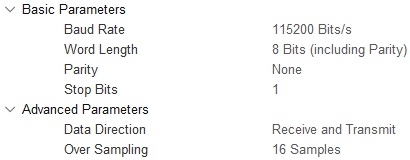
\includegraphics[width=100mm]{Rysunki/Rozdzial4/usart3_parameters.jpg}
    \caption{USART3 and USART6 configuration}
    \label{fig:my_label}
\end{figure}

The next step consists of setting up the HSE in the System Core section of the RRC tab in the BYPASS mode, similarly as in case of the Ethernet interface, in order to use the ST-Link clock signal for clocking the microcontroller.

\begin{figure}[!ht]
    \centering
    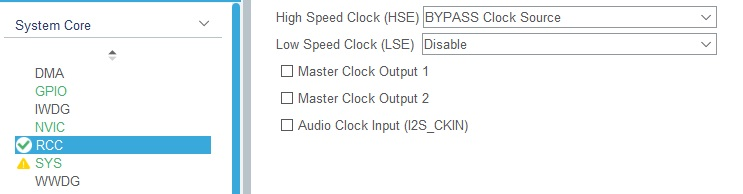
\includegraphics[width=155mm]{Rysunki/Rozdzial4/rcc_wifi.jpg}
    \caption{HSE clock setup}
    \label{fig:my_label}
\end{figure}

In the \emph{Clock Configuration} tab, the system clock frequency was set via the configurator to 180 MHz, as shown on figure 4.15.

\begin{figure}[!ht]
    \centering
    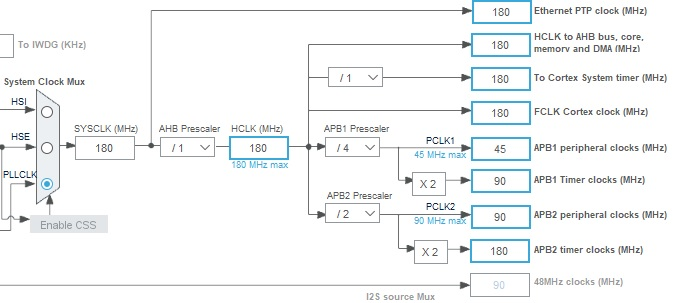
\includegraphics[width=155mm]{Rysunki/Rozdzial4/wifi_zegary.jpg}
    \caption{Target frequencies in the clock manager}
    \label{fig:my_label}
\end{figure}

The last steop of the configuration process required configuring one of the GPIO ports in the output mode, in order to control the \emph{enable} line of the Wi-Fi module. In order to activate the module and enable operating it, the line required a high logical state. Line PB3 was used for this purpose, keeping its default parameters, for which the monitoring and modification options are available in the GPIO tab of the \emph{System Core} section. They were presented on figures 4.16 and 4.17.

\begin{figure}[!ht]
    \centering
    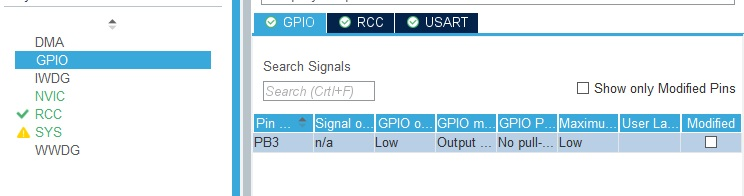
\includegraphics[width=155mm]{Rysunki/Rozdzial4/gpio_pb3.jpg}
    \caption{Configured GPIO lines}
    \label{fig:my_label}
\end{figure}

\begin{figure}[!ht]
    \centering
    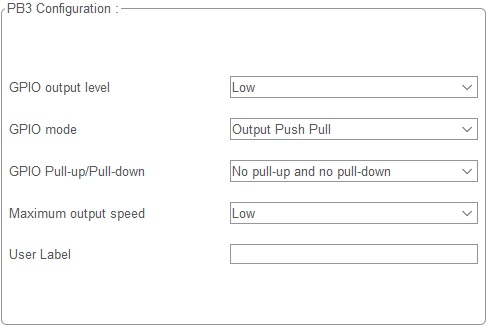
\includegraphics[width=100mm]{Rysunki/Rozdzial4/gpio_pb3_2.jpg}
    \caption{PB3 line parameters}
    \label{fig:my_label}
\end{figure}

The ESP8266 module contains a functioning implementation of the TCP/IP stack, and as such enabling the LwIP stack in the platform configurator was not required. Based on this configuration, the source was generated, which was subsequently extended with snippets that configure the Wi-Fi module and implement the echo server functionality. Listing 4.18 shows the contents of the \textit{main()} function and the globally available elements.

\cppcode{Listingi/WiFi_main.c}{\textit{main()} function and global elements}

The global elements were defined as:

\begin{itemize}
    \item [$\bullet$] character buffer for reception from the Wi-Fi module;
    \item [$\bullet$] character buffer for formatted message to be sent back;
    \item [$\bullet$] macro defining the Wi-Fi configuration commands amount;
    \item [$\bullet$] look up table containing the commands for configuring the Wi-Fi module.
\end{itemize}

The result of each of the configuration commands was described via comments inside listing 4.18. For privacy protection reasons, the password contained in the listing for the \textit{AT+CWJAP} command was censored with asterisks.

The \textit{main()} function consists of several key sections. The first one is the generated configuration section for each of the interfaces and microcontroller components, such as GPIO, system clock and USART interfaces. This section was extended with setting the PB3 line connected to the \emph{enable} input of the Wi-Fi module into high logical state.

Second section is the configuration loop. Is is tasked with performing the reset and configuration of the Wi-Fi module in a way which enables connection and two-way transmission of messages. These commands are subsequently:

\newpage

\begin{itemize}
    \item [$\bullet$] \emph{AT+RST} - module reset;
    \item [$\bullet$] \emph{ATE0} - disabling the configuration commands echo;
    \item [$\bullet$] \emph{AT} - communication test with the module;
    \item [$\bullet$] \emph{AT+GMR} - acquiring module firmware version;
    \item [$\bullet$] \emph{AT+CWMODE=1} - configuring the module into client mode;
    \item [$\bullet$] \emph{AT+CIPMODE=0} - configuring the received message format as "+IPD,\newline<channel>,<byte count>,<data>";
    \item [$\bullet$] \emph{AT+CIPMUX=1} - enabling multiconnectivity;
    \item [$\bullet$] \emph{AT+CIPSERVER=1,7} - configuring the server on port 7;
    \item [$\bullet$] \emph{AT+CWMODE=?} - verifying the operating mode;
    \item [$\bullet$] \emph{AT+CWJAP=<SSID>,<password>} - connecting to the Wi-Fi network;
    \item [$\bullet$] \emph{AT+CIPSTA?} - querrying connection status;
    \item [$\bullet$] \emph{AT+CIFSR} - acquiring the server IP address;
\end{itemize}

After sending the module reset command, the microcontroller awaits 1 second before transmitting subsequent commands. Each transmission consists of sending the command to the module, clearing the reception buffer using the \textit{clr\char`_buffer()} function presented on listing 4.19, and receiving the feedback from the module. After the \emph{AT+CWJAP} querry, the microcontroller awaits acquiring an IP address from DHCP in 1-second intervals, by querrying the connection status via the \textit{is\char`_busy()} function shown on listing 4.20. As long as the status informs that the module is busy, the process is repeated. Feedback from the module is relayed to the overseeing computer via the serial port. 

\cppcode{Listingi/clr_buffer.c}{Reception buffer clear function}

\newpage
\cppcode{Listingi/is_busy.c}{Wi-Fi module state querry function}

The third section of the \textit{main()} function contains the operating loop, which acts as the echo server functionality. Inside it, a reception buffer is cleared and data is read from the module when an event such as establishing connection or data reception occurs. In case of receiving a non-empty feedback message, the echo functionality is prepared inside the \textit{prepare\char`_echo()} function, which code can be found in listing 4.21.

\cppcode{Listingi/prepare_echo.c}{Preparing the echo functionality}

If the received feedback message starts with the "+IPD" sequence, the program extracts the number of bytes and its content in order to properly format it and prepare it for sending back. Readiness for sending is stated by the \textit{ready\char`_to\char`_send} flag. In case of extracting the message, a "send data" command is transmitted, followed by the message content in the third section of the \textit{main()} function.\ After performing the echo transmission, the \textit{ready\char`_to\char`_send} flag is reset/

%=================================================================================================
\section{Solution tests}

\subsection{Ethernet interface}

During the testing phase, following functionalities were validated:

\begin{itemize}
    \item [$\bullet$] communication with the overseeing computer via the serial port, acquiring information about the MAC address and the connection state; 
    \item [$\bullet$] exchanging the ping via Windows command prompt;
    \item [$\bullet$] connection and two-way exchange via Hercules SETUP Utility software.
\end{itemize}

Figures 4.18, 4.19 and 4.20 showcase the results of carried out tests. The first action included acquiring the IP address of the module via USART serial interface. Subsequently, the connection could be validated using the \emph{ping} command, and the echo server functionality could be verified using the Hercules SETUP Utility. All of the tests were successful, confirming the proper functioning of the Ethernet network interface. 

\begin{figure}[!ht]
    \centering
    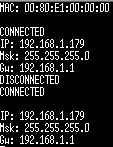
\includegraphics[width=50mm]{Rysunki/Rozdzial4/usart_ethernet.jpg}
    \caption{Serial port communication}
    \label{fig:my_label}
\end{figure}

\begin{figure}[!ht]
    \centering
    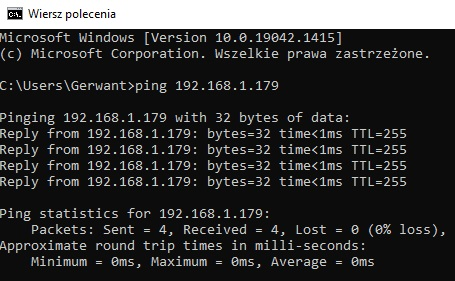
\includegraphics[width=130mm]{Rysunki/Rozdzial4/ping_ethernet.jpg}
    \caption{Verifying connection via ping}
    \label{fig:my_label}
\end{figure}

\begin{figure}[!ht]
    \centering
    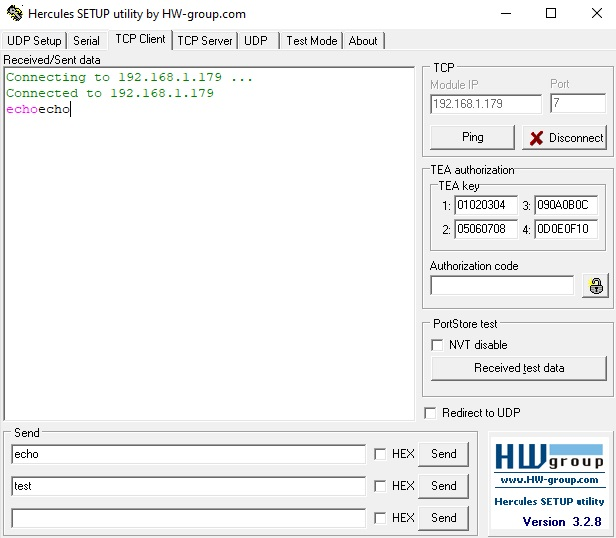
\includegraphics[width=110mm]{Rysunki/Rozdzial4/hercules_ethernet.jpg}
    \caption{Two-way communication validation using Hercules SETUP Utility}
    \label{fig:my_label}
\end{figure}

\newpage
\subsection{Wi-Fi wireless interface}

The figure 4.21 showcases a picture of the prepared circuit. Similarly to the Ethernet interface, the same set of tests was performed. Due to the reset of the device, on picture 4.22 some unreadable messages can be seen, caused by the different speed of transmission during the bootloader execution of the module. Just like in the case of the Ethernet interface, first the IP address of the module was acquired via an USART interface, which was shown on figure 4.22 and 4.23. Subsequently communication tests were carried out using the \emph{ping} command, which is shown on figure 4.24 and the echo server functionality using the Hercules SETUP Utility software shown on figure 4.25. All tests were successful.

\begin{figure}[!ht]
    \centering
    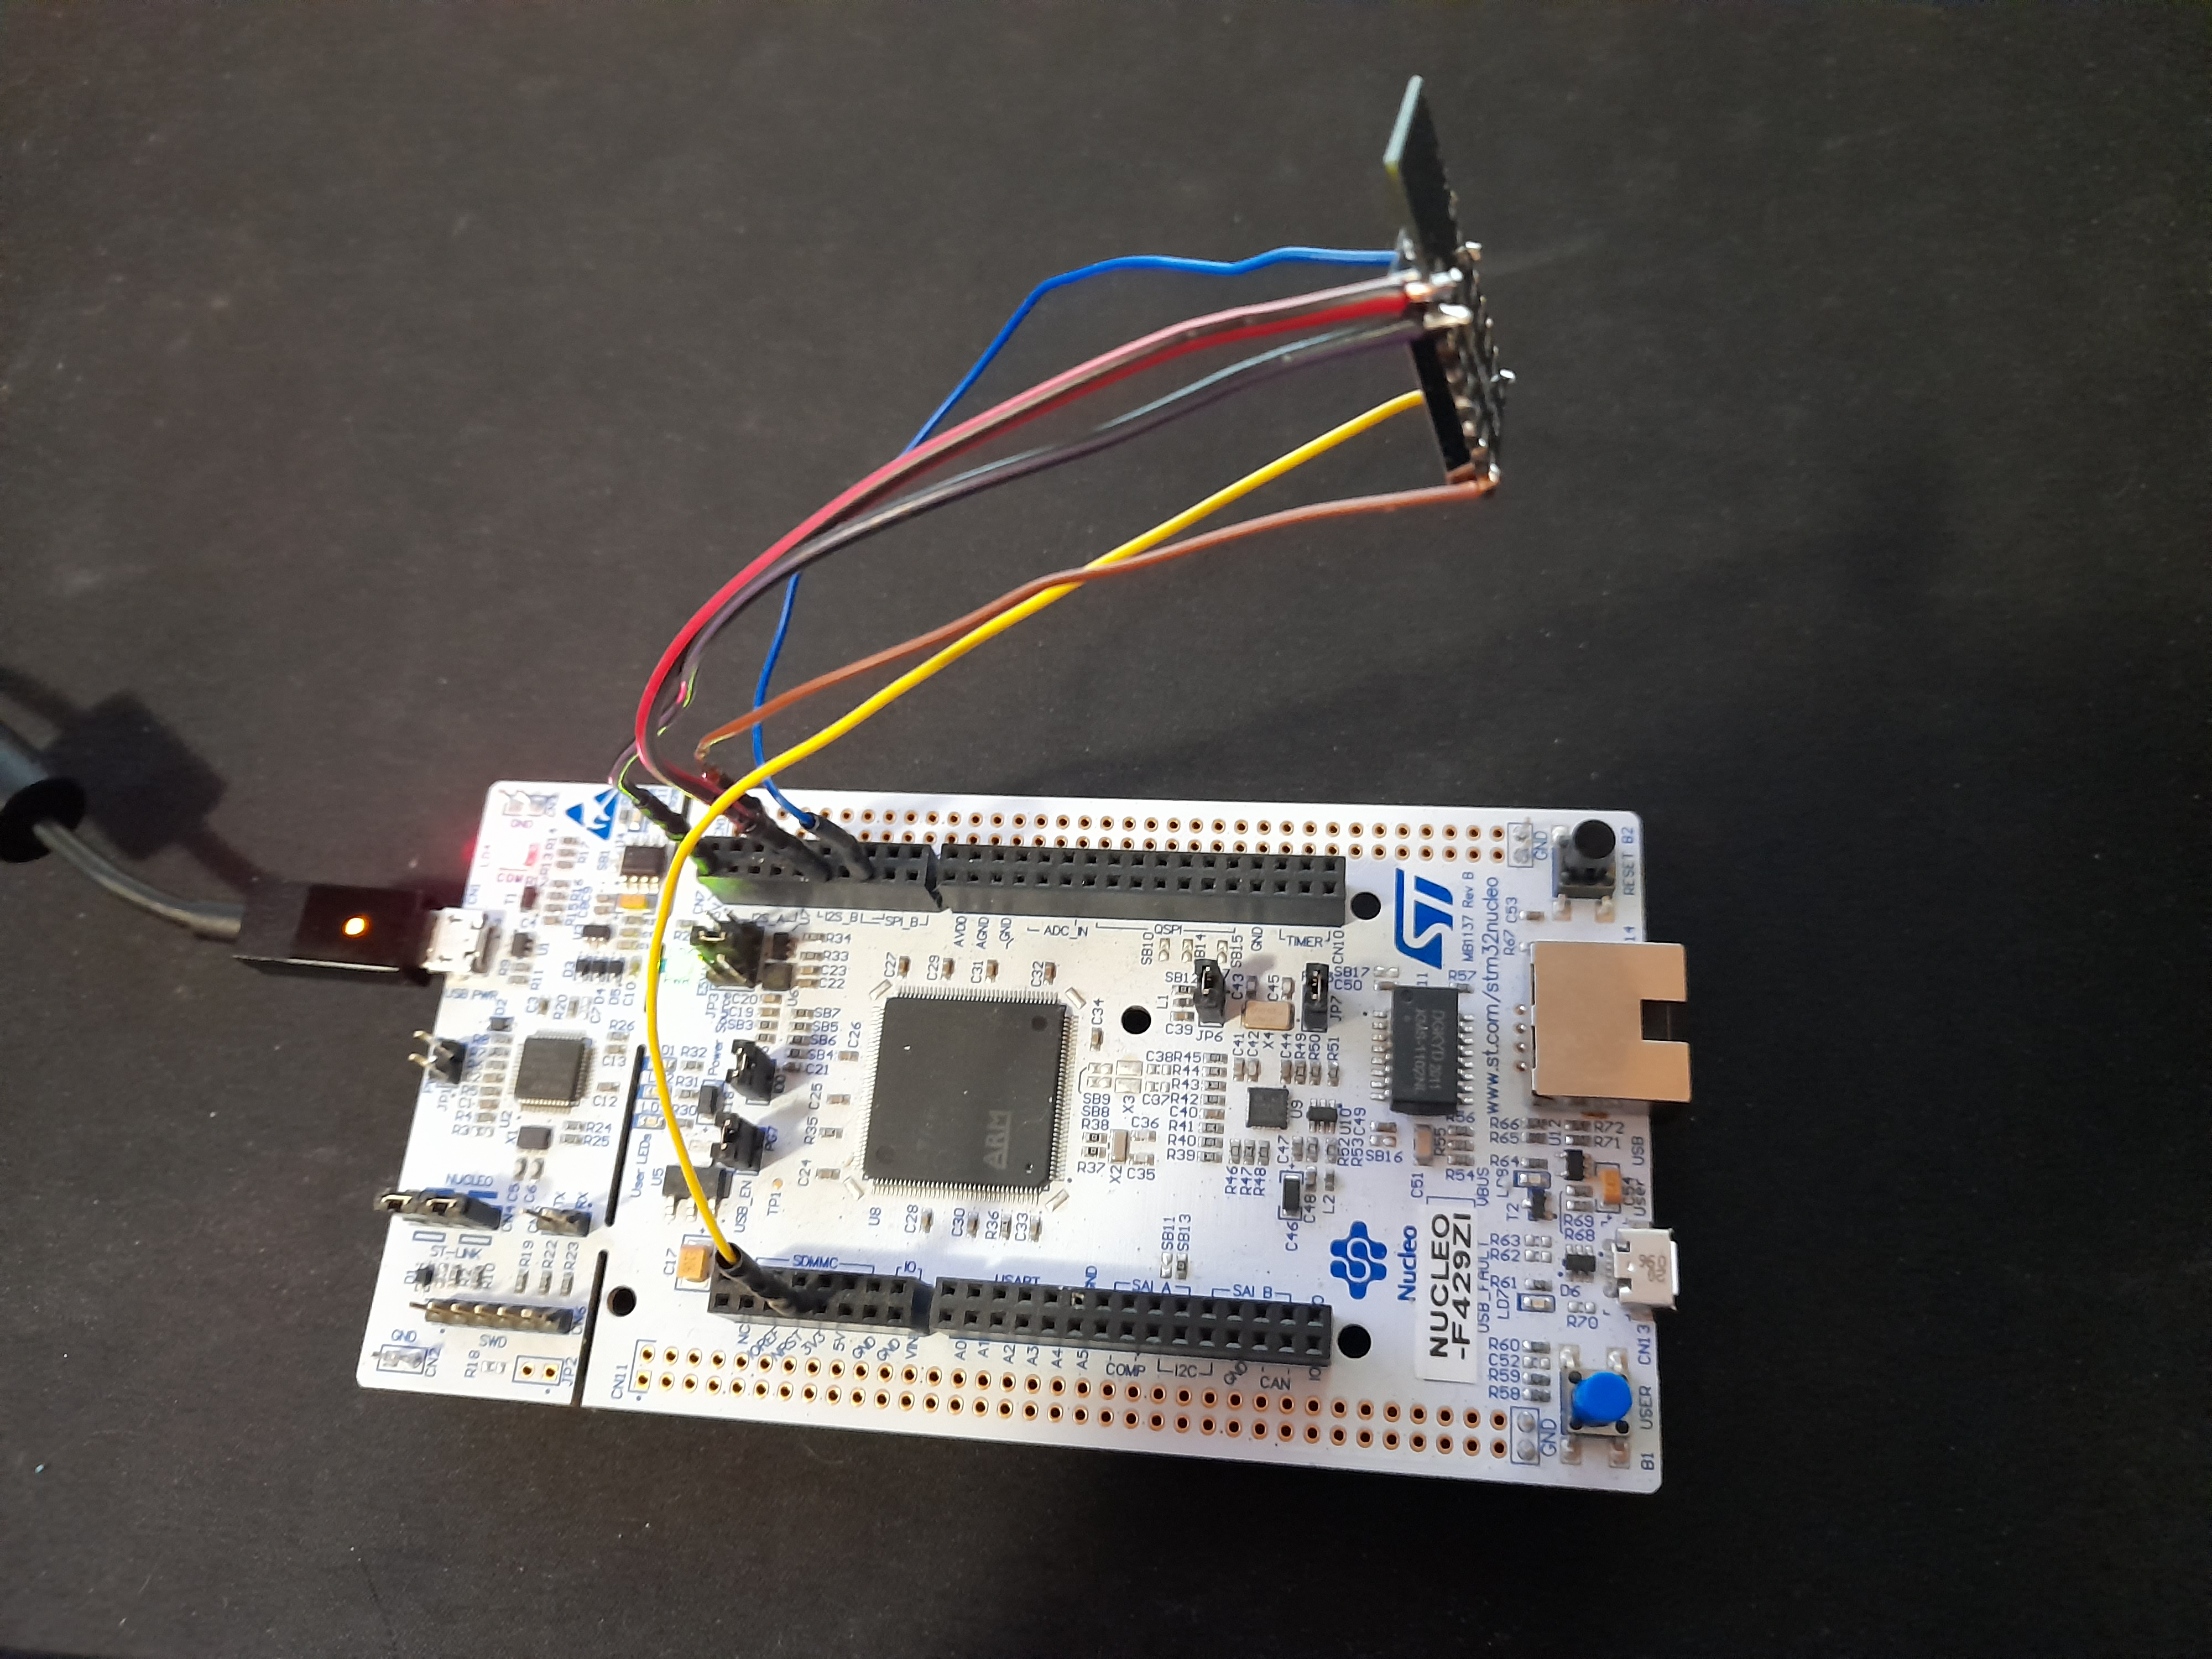
\includegraphics[width=80mm]{Rysunki/Rozdzial4/modul.jpg}
    \caption{Constructed circuit}
    \label{fig:my_label}
\end{figure}

\begin{figure}[!ht]
\begin{minipage}[b]{0.4\textwidth}
    \centering
    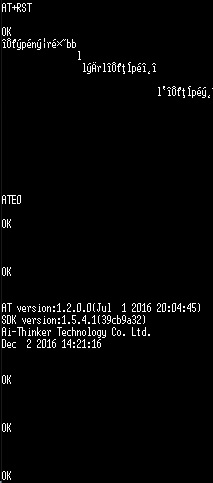
\includegraphics[width=50mm]{Rysunki/Rozdzial4/wifi_usart_1.jpg}
    \caption{Communication with overseeing computer pt. 1}
  \end{minipage}
  \hfill
  \begin{minipage}[b]{0.4\textwidth}
    \centering
    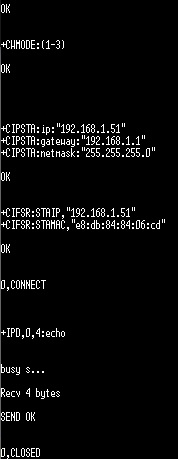
\includegraphics[width=50mm]{Rysunki/Rozdzial4/wifi_usart_2.jpg}
    \caption{Communication with overseeing computer pt. 2}
  \end{minipage}
\end{figure}


\begin{figure}[!ht]
    \centering
    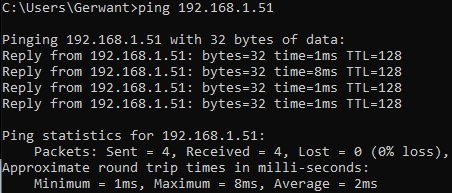
\includegraphics[width=120mm]{Rysunki/Rozdzial4/wifi_ping.jpg}
    \caption{Testing connectivity using \textit{ping}}
    \label{fig:my_label}
\end{figure}

\begin{figure}[!ht]
    \centering
    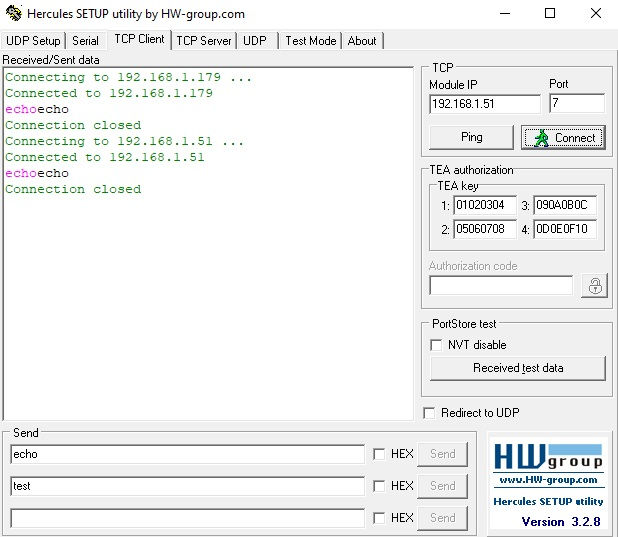
\includegraphics[width=130mm]{Rysunki/Rozdzial4/wifi_hercules.jpg}
    \caption{Two-sided communication using Hercules SETUP Utility software}
    \label{fig:my_label}
\end{figure}

